\chapter{线性空间}
\section{线性空间}
\begin{definition}{线性空间}{linear space}
	定义域$\FF$上的线性空间(linear space)~$V$是具有加法$+:V\times V\to V$和数乘$\cdot:\FF\times V\to V$运算且满足以下公理的集合。
	\begin{compactenum}
		\item 加法交换律\qqqquad\quad~$x+y=y+x;$
		\item 加法结合律\qqqquad\quad~$x+(y+z)=(x+y)+z;$
		\item 加法零元\qqqquad\qquad~$x+0=x;$
		\item 加法逆元\qqqquad\qquad~$x+(-x)=0;$
		\item 数乘单位元\qqqquad\quad~$1x=x;$
		\item 数乘结合律\qqqquad\quad~$(c_1c_2)x=c_1(c_2x);$
		\item 数乘对向量的分配律\quad$c(x+y)=cx+cy;$
		\item 数乘对标量的分配律\quad$(c_1+c_2)x=c_1x+c_2x.$
	\end{compactenum}
\end{definition}
比如$\RR^n$和$\CC^n$都是线性空间。
\begin{definition}{子空间}{subspace}
	线性空间$V$的子空间(subspace)~$V_s\subset V$,且对于加法和数乘封闭:$\forall v,w\in V_s,\forall c\in\FF$
	\[
		v+w\in V_s,\quad cv\in V_s,
	\]
	即子空间中元素的线性组合都在同一个子空间。
\end{definition}
子空间必然包含零向量。因为若$v\in\FF$,则$v+(-v)=0\in\FF.$

一般来说,线性空间$V$的子集$S$不是子空间,但我们可以从$S$中构造出子空间。

\begin{definition}{线性扩张}{linear span}
	$S$的线性扩张(linear span)~$\spn(S)$是$S$中向量的所有线性组合的集合。$\spn(S)$是$V$的子空间。
\end{definition}
\section{线性独立、基和维度}
\begin{definition}{线性独立}{linear independent}
	$n$个向量$\{v_i\}$是线性独立的(linear independent),当且仅当
	\[
		\sum_{i=1}^nx_iv_i=0,
	\]
	只在$x_i=0$时成立,即只有零解。$n$个向量$\{v_i\}$不是线性独立,那么他们是线性相关的(linear correlate)。
	
	等价描述:集合中每一个向量都不能写成其它向量的线性组合。
\end{definition}
向量是否线性独立同数域的选择密切相关。
\begin{definition}{线性空间的基}{base}
	线性空间$V$的基(base)是一组线性无关的向量$\{v_i\}$,并且他们张成整个线性空间$V$。
\end{definition}
$\{e_i\}$构成$\RR^n$的一组基。
\begin{definition}{线性空间的维度}{dimension}
	线性空间的维度(dimension)~$\dim(V)$等于任一组基中向量的个数。
\end{definition}
\begin{theorem}{维度的确定性}{certainty of dimension}
	线性空间的维度和基的选取无关。
\end{theorem}
\begin{proof}
	若线性空间$V$存在两组基$\{v_1,\ldots,v_m\},\{w_1,\ldots,w_n\}$元素个数不等,不妨设$n>m$。
	
	因为$\{w_i\}$是基,$\{v_i\}$可以被表示为其线性组合
	\[
		v_i=\sum_{j=1}^nw_ja_{ji},\quad\forall i.
	\]
	考虑线性组合
	\[
		\sum_{i=1}^mx_iv_i=\sum_{i=1}^m\sum_{j=1}^nx_iw_ja_{ji}=0.
	\]
	因为$\{w_i\}$线性无关,故
	\[
		\sum_{i=1}^ma_{ji}x_i=0,\quad\forall j,
	\]
	但是其未知数的个数$m>$方程的个数$n$,系数矩阵一定有自由列,所以有非零解。这与$\{v_i\}$线性无关矛盾!故$m=n.$
\end{proof}

\begin{theorem}{}{}
	若$\forall v\in V_1$可以写成$V_2$中向量的线性组合,则$\dim(V_1)\leqslant\dim(V_2)$。
\end{theorem}
这个定理是trivial的,证明留给读者。

\begin{definition}{变换矩阵}{transfomation matrix}
	不同基之间的变换相应的矩阵称为变换矩阵(transfomation matrix)。
\end{definition}

\section{矩阵\textit{A}的四个子空间}
对于$m\times n$矩阵$A$,可以由其得到四个子空间:列空间$\C(A)$、行空间$\C(A\tp)$、零空间$\N(A)$和左零空间$\N(A\tp)$。
\begin{definition}{列空间}{column space}
	矩阵$A$的列空间(column space)~$\C(A)$是$A$的所有列的线性组合的集合。
	\tcblower
	类似的,行空间(row space)是所有行的线性组合的集合,%由于转置并不影响性质,行空间
	可以用$\C(A\tp)$表示。
\end{definition}
不难验证,$\C(A)$是$\RR^n$的子空间,$\C(A\tp)$是$\RR^m$的子空间。

线性方程组$Ax=b$有解等价于$b\in\C(A)$。
\begin{definition}{零空间}{null space}
	矩阵$A$的零空间(null space)~$\N(A)$是$Ax=0$所有解$x$构成的线性空间。
	\tcblower
	类似的,左零空间(left null space)是$x\tp A=0$所有解$x$构成的线性空间,可用$\N(A\tp)$表示。
\end{definition}
$\N(A)$是$\RR^m$的子空间,$\N(A\tp)$是$\RR^n$的子空间。
\begin{example}{子空间的基}{}
	显然$\N(A)=\N\bigkh{\rrem(A)}$,而$\N\bigkh{\rrem(A)}$中的基可以这样给出:
	\begin{compactitem}
		\item 每个自由列给出一个向量,因此$\dim\bigkh{\N(A)}=\rrem(A)$中自由列的数量;
		\item 自由列$j$对应向量$x$中,$x_j=1$,$x$对应其他自由列分量为0,对应主列$i$分量$x_i=-\rrem(A)_{ij}$
	\end{compactitem}
	\tcblower
	$\rrem(A)$所有主列构成$\C(A)$一组基。
\end{example}
\section{矩阵的秩、线性代数基本定理}
\begin{definition}{矩阵的秩}{rank}
	矩阵$A$的秩(rank)~$\rank(A)$定义为行空间或列空间的维数%\footnote{后面很快会证明行空间列空间维数相等。}:
	\[
		\rank(A):=\dim\bigkh{\C(A)}=\dim\bigkh{\C(A\tp)}.
	\]
	进而可定义行满秩矩阵(full row rank matrix)满足
	\[
		\rank(A)=\row(A).
	\]
	列满秩矩阵(full column rank matrix)定义类似。
\end{definition}
\paragraph{线性方程组$Ax=0$的完整解}考虑线性方程组$Ax=b$,通解
\[
	x=x_{\mathrm p}+x_{\mathrm n},
\]
其中$x_{\mathrm n}\in\N(A)$,特解$x_{\mathrm p}$可以从约化的增广矩阵$[\rrem(A),b']$中选取:自由列$i$对应$x_{{\mathrm p}i}=0$,若主元列$i$中的1在第$j$行,则$x_{{\mathrm p}i}=b'_j.$
\begin{itemize}
	\item 若$A$列满秩,$\rrem(A)$没有自由列,$\N(A)=\{0\}$,有唯一解($b\in\C(A)$)或无解;
	\item 若$A$行满秩,$\rrem(A)$没有零行,$\C(A)=\RR^m$,$\forall b$都有解,有唯一解或无穷多解。
\end{itemize}
\paragraph{四个子空间的维度}已经知道,初等行变换就是用初等矩阵$E$左乘$A$,相应的,列变换就是$E$右乘$A$。
\begin{theorem}{初等变换和子空间}{}
	\begin{compactitem}
		\item $\N(A)=\N(EA)$,因为
		\[
			Ax=0\iff EAx=0.
		\]
		\item $\dim\bigkh{\C(A)}=\dim\bigkh{\C(EA)}$,因为
		\[
			\{v_i\}\text{~是~}\C(A)\text{~一组基}\iff\{Ev_i\}\text{~是~}\C(EA)\text{~一组基}.
		\]
		\item $\C(A)=\C(AE)$,因为
		\[
			AE\text{~的每一列}\in\C(A)\text{~且~}A=(AE)E\iv\text{~的每一列}\in\C(AE)
		\]
		\item $\dim\bigkh{\N(A)}=\dim\bigkh{\N(AE)}$,因为可由
		\[
			Ax=0\iff AE(E\iv x)=0,
		\]
		推出
		\[
			\{v_i\}\text{~是~}\N(A)\text{~一组基}\iff\{E\iv v_i\}\text{~是~}\N(AE)\text{~一组基}
		\]
	\end{compactitem}
\end{theorem}
即,矩阵$A$在初等变换下,$\dim\bigkh{\C(A)}$和$\dim\bigkh{\N(A)}$均不变,而行变换下$\N(A)$不变,列变换下$\C(A)$不变。

因此,可以将$A$先由行变换为$\rrem(A)$,再列变换为
\[
	\tilde I=\begin{bmatrix}
		I_r&0\\0&0
	\end{bmatrix}.
\]
显然,$\tilde I$的行秩$\dim\bigkh{\C(\tilde I\tp)}=$列秩$\dim\bigkh{\C(\tilde I)}=r$,且
\begin{align*}
	\dim\bigkh{\C(\tilde I\tp)}+\dim\bigkh{\N(\tilde I)}&=n;\\
	\dim\bigkh{\C(\tilde I)}+\dim\bigkh{\N(\tilde I\tp)}&=m.
\end{align*}
以上的这些量在初等变化下都不变,故
\begin{theorem}{线性代数基本定理·一}{fundamental theorems of linear algebra I}
	\begin{compactenum}
		\item 行秩=列秩:$\dim\bigkh{\C(A)}=\dim\bigkh{\C(A\tp)};$
		\item $\dim\bigkh{\C(A\tp)}+\dim\bigkh{\N(A)}=n;$
		\item $\dim\bigkh{\C(A)}+\dim\bigkh{\N(A\tp)}=m.$
	\end{compactenum}
\end{theorem}
\begin{corollary}
	方阵$A$可逆$\iff A$满秩。
\end{corollary}
\begin{center}
    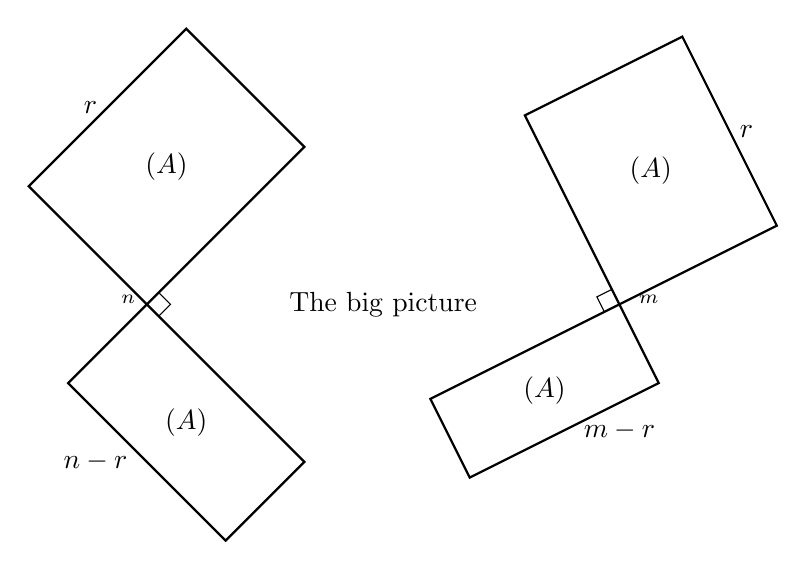
\begin{tikzpicture}
        \node at(3, 0){The big picture};
        \draw[thick](0, 0)node[left]{$\RR^n$}--(2, 2)--(.5, 3.5)--(-1.5, 1.5)node[midway, left]{$r$}--(2, -2)--(1, -3)--(-1, -1)node[midway, left]{$n-r~$}--cycle;
        \draw(.15, .15)--(.3, 0)--(.15, -.15);
        \node at(.25, 1.75){$\C(A\tp)$};
        \node at(.5, -1.5){$\N(A)$};
        \draw[thick](6, 0)node[right]{$~\RR^m$}--(8, 1)--(6.8, 3.4)node[midway, right]{$r$}--(4.8, 2.4)--(6.5, -1)--(4.1, -2.2)node[midway, right]{$~m-r$}--(3.6, -1.2)--cycle; % +6
        \draw(5.905, .19)--(5.715, .095)--(5.81, -.095); % .03√10
        \node at(6.4, 1.7){$\C(A)$};
        \node at(5.05, -1.1){$\N(A\tp)$};
    \end{tikzpicture}
    \captionof{figure}{$A$的四个子空间}
\end{center}
\paragraph{矩阵的秩的不等式}参考:\url{https://zhuanlan.zhihu.com/p/55206421}
\begin{theorem}{}{}
	对于矩阵$A,B$有
	\begin{equation}
		\rank(A+B)\geq\rank(A)+\rank(B).
	\end{equation}
\end{theorem}
\begin{proof}
	设$A,B$的列空间的一组基分别为$\{a_1,\ldots,a_{\rank(A)}\}$和$\{b_1,\ldots,b_{\rank(B)}\}$,则$A+B$中的列必然可以由$\{a_1,\ldots,a_{\rank(A)},b_1,\ldots,b_{\rank(B)}\}$的线性组合表示出,故不等式成立。
\end{proof}
\begin{theorem}{Sylvester不等式}{Sylvester inequality}
	对$n$阶方阵$A,B$有
	\begin{equation}
		\rank(AB)\geq\rank(A)+\rank(B)-n.
	\end{equation}
\end{theorem}
\begin{proof}
	注意到
	\[
		\rank(AB)+n=\rank\biggkh{\begin{bmatrix}
			I_n\\ &AB
		\end{bmatrix}}=\rank\biggkh{\begin{bmatrix}
			I_n&-B\\A
		\end{bmatrix}}\geq\rank(A)+\rank(B).\qedhere
	\]
\end{proof}

\begin{theorem}{Frobenius秩不等式}{Frobenius rank inequality}
	对于矩阵$A,B,C$,有
	\begin{equation}
		\rank(ABC)\geq\rank(AB)+\rank(BC)-\rank(B).
	\end{equation}
\end{theorem}
\begin{proof}
	注意到
	\begin{align*}
		\rank(ABC)+\rank(B)&=\rank\biggkh{\begin{bmatrix}
			B\\ &ABC
		\end{bmatrix}}\\
		&=\rank\biggkh{\begin{bmatrix}
			BC&B\\ &AB
		\end{bmatrix}}\geq\rank(AB)+\rank(BC).\qedhere
	\end{align*}
\end{proof}

